\subsection{Human to Humanoid Robot Kinematic Mapping}\label{sec:sec:mocap}

Motion capture systems are increasingly developed and used as important tool insports training and roboticsto generate human-like motion. 
There exist enormous robotics researches that reply on motion capture data. 
From the sport training perspective, the motion capture system is utilized for example to monitor the movement and reconstruct the movement on a synthetic model. 
[mirabella] The focus is on kinematics analysis to improve and transmitting skill in a sport [1][2][3][4]. 
The key research area in robotics is more of retargeting and execution on the robot than kinematics analysis of the motion data.  
Various approaches for generation of human-like motion for humanoid robots were proposed [qiang][pollard][stefan]. 
Most of the approaches use 3D marker positions as the starting point of data collection.
Stefan et al attempt to use an intermediate model(Master Motor Map) to decouple motion capture data from further post-processing tasks. 
However this added in another conversion to the overall process which causes data lose. 
On the other hand, the motion capture system we adopted auto-generates a lower DoF skeleton from the 3D marker clouds. 
This makes the data collected closer to what we want, and can be seen as a non-physical intermediate model which converts high DoF human motion to lower DoF skeleton motion generated by motion capture system. 
%As many of the mentioned researches above are done in case of relatively slow motion, the high-speed throwing motion which requires high dynamic stability becomes a main concern. The ground contact constraints proposed in [qiang] points out the key issue in the dynamic stability.

Our method for mapping human motion to humanoid motion incorporates the following stages: 1) Human motion capture. 2) Kinematics mapping. 3) Dynamic mapping. 
A motion capture system used in the experiment consists of eighteen cameras with VGA resolution running at 100fps. 
It is able to record the full body motion using thirty-eight reflective markers placed on the actor's body. 
The system creates a 3D cloud of marker points at the rate of 100hz in sub-millimeter precision. 
These 3D points are labeled and mapped to a skeleton of twenty two bones with specifications of the actor's body. 
The skeleton is a human body representation in the motion capture system. 
In this way, the position and the rotation of the bones are obtained in each frame.
The rotation of each bone in the local frame is given in quaternions.% with respect to the end tip of the previous bone.
Kinematics mapping has to resolve three key issues: 
\begin{itemize}
	\item The difference in the total degree of freedom (DOF). 
	\item	The difference in the kinematics descriptions. 
	\item	Kinematic constraints for the robot.
\end{itemize}

The difference in number of bones (linkages) as well as the DOF for each joint caused the difference in the total DOF. 
In reality, all anatomic joints for a human have six DOF []. 
Humans also have soft tissues and vertebra that create more DOF []. 
The skeleton generated does not have soft tissues, it replaced the vertebra with three bones and Hubo has only one DOF(yaw) in between the neck and the hip. 
The key to a successful kinematics mapping will then be to deliver the main information as close as possible and estimate the rest. 
Hence for the underhand throwing motion, the yaw angle of Hubo's waist is the combination of the two joints' yaw angles of the human skeleton.  %% what two joints
The difference in kinematics descriptions lies in the joint configuration. 
(The gross movement of the limb segments interconnected by joints where for the Jaemi HUBO the relative joint rotation is described by adopting the Eulerian angle system, for the human skeleton, Quaternions are used.) 
For Hubo, the finite rotation of joint in the two bone segments is sequence dependent while for human skeleton, the associated three-dimensional finite rotation is sequence independent.
Unlike the generated skeleton in the motion capture system where each joint has multiple DOF, Hubo is constructed with single DOF joints. This makes the joint orientations follow a specific sequence during conversion. For example, from the shoulder to the upper arm, the sequence for shoulder joints is pitch, roll and yaw.  If we move roll prior to pitch, it won't affect the pitch axis but will change the yaw axis.

\begin{figure}[t]
  \centering
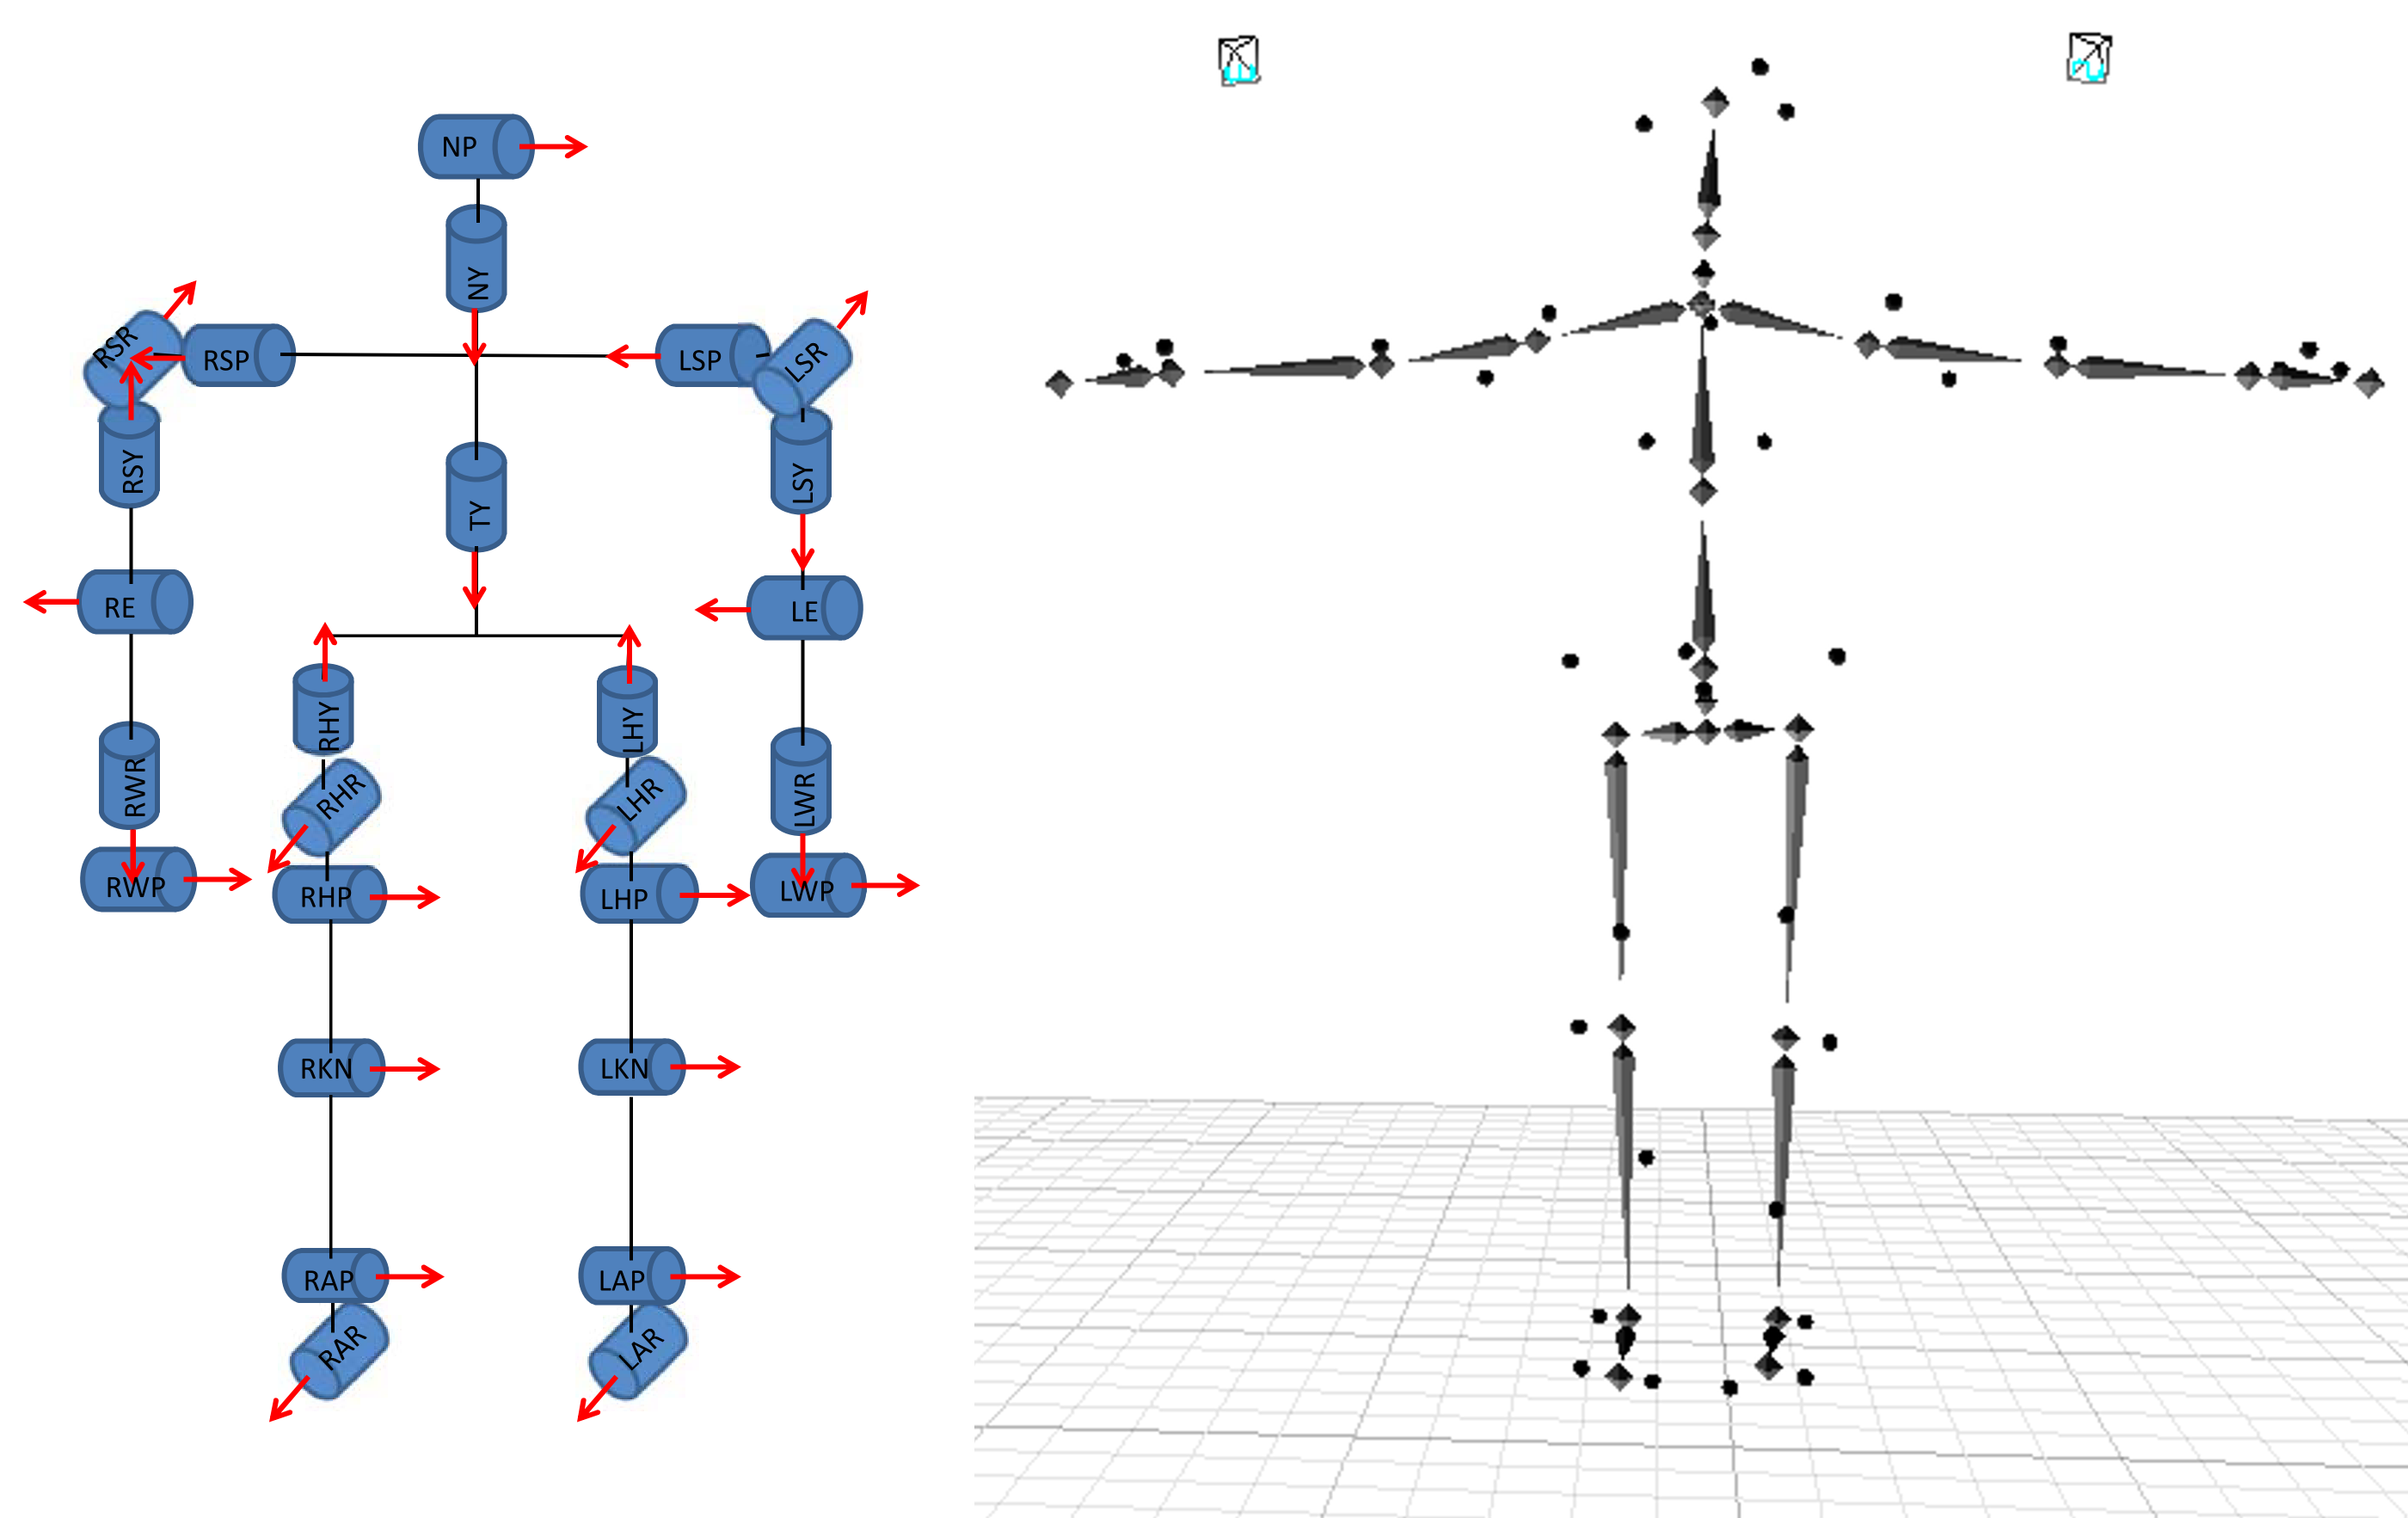
\includegraphics[width=1.0\columnwidth]{./pix/mocapJoints.png}
  \caption{Left: Jaemi Hubo joint order and orientation using right hand rule.  Right: Skeleton generated from motion capture system.  Each joint has three degrees of freedom described via Quaternions in the local frame.}
  \label{fig:mocap-joints}
\end{figure}

Kinematics constraints for the robot include joint angle range and limb contact. 
The kinematics mapping starts from the conversion from quaternions used in motion capture generated skeleton to Euler angles used in Hubo. 
We mainly solve two problems during conversion.  1) Unlike quaternion representation, Euler angles are determined by 24 conventions.  The joint orientation matters for the robot.  Therefore to generate the mapping for a given set of Euler angles, we map rotating axis ri, rj, rk to reference axis i, j, k in the appropriate order.  2) Singularities are generated in conversion from quaternions to Eulerian angle system. When the pitch angle approaches +90 degrees, singularities may occur. We use two methods to avoid singularities. First, use an approximated function for the singularity zone. Second, choose a favorable sequence for joints that have less than three orientations for the robot.
Convention zxy: 
double test = qw*qx + qy*qz;
if (test > 0.499) // singularity at north pole
		yaw = (float) 2.0f * atan2(qy,qw);
		pitch = 3.14159265f/2.0f;
		roll = 0;

if (test < -0.499) // singularity at south pole
		yaw = (float) -2.0f * atan2(qy,qw);
		pitch = - 3.14159265f/2.0f;
		roll = 0;
        

    double sqx = qx*qx;
    double sqy = qy*qy;
    double sqz = qz*qz;
yaw = (float) atan2((double)2.0*qw*qz-2.0*qx*qy , (double)1 - 2.0*sqz - 2.0*sqx);
pitch = (float)asin(2.0*test);
roll = (float) atan2((double)2.0*qw*qy-2.0*qx*qz , (double)1.0 - 2.0*sqy - 2.0*sqx);


